\documentclass[a4paper]{article}
\pagestyle{plain}
%\usepackage[cp1251]{inputenc}
\usepackage[utf8]{inputenc}
\usepackage[english,ukrainian]{babel}
\usepackage[pdftex]{graphicx}
\usepackage{amsmath,amssymb}
\usepackage[colorlinks=true, allcolors=blue]{hyperref}

\paperwidth=210mm
\paperheight=297mm

\hoffset=0.0mm 		% By default offset from paper edge is 1 inch, this will set it to 25mm
\voffset=-5.4mm		% By default offset from paper edge is 1 inch, this will set it to 20mm

\oddsidemargin=0mm	% This will add nothing to hoffset
\evensidemargin=0mm	% This will add nothing to hoffset
\topmargin=0mm
\headheight=0mm
\headsep=0mm

\textwidth=170mm
\textheight=237mm


\begin{document}
\title{Як побудовані сучасні цифрові дисплеї}
\author{\textsl{Сукованченко Дмитро}}
\date{\vspace*{-6ex}}
\maketitle
\begin{center} 
{\small Група ІПС-31, курс 3, факультет кібернетики\\
{\tt dmitro-sv@knu.ua}}
\end{center}


\section{Що таке цифровий дисплей}

Дисплей (англ. display «показувати») — электроний пристрій, який виводить на экран текстову або графічну інформацію. Використовуеться для надання інформації від "заліза" до людини у зрозумілій для неї формі.

Найчастіше можна побачити в телевізорах, моніторах комп'ютерів, ноутбуках, телефонах, навігаторфах, фітнес-трекерах або смарт годинниках, банківських та платіжних терміналах, бігбордах та вуличній рекламі, різних фізичних приладах для вимірювань.

Основними різновидами є електронно-променеві, жидкокристалічні та плазмені дисплеї

\section{Електронно-променеві прилади}

Пристрої в яких використовується потік електронів, сформований у формі одиночного пучка або кількох пучків, керовані як за інтенсивністю (струму пучка), так і за положенням пучка в просторі і ці пучки взаємодіють з нерухомою мішенню (екраном) прилад, що при високих частотах дозволяє побачити необхідне зображення.

\begin{figure}[ht]
\centering{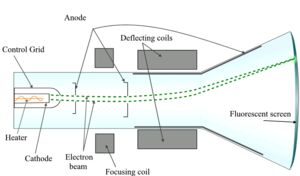
\includegraphics[width=0.5\textwidth]{rayTube.PNG}}
\caption{Електронно-променева трубка з використанням електромагнітного фокусування та відхилення}
\end{figure}


\section{Рідкокристалічний дисплеї}

Пристрої що складаються з великої кількості рідких кристалів, за допомогою яких зображення розбивають на pixels (англ picture elements - "елементи зображення").

Існує багато варіантів саме цього типу (IPS, WLED, AMOLED, VA, DSTN, STN, AFFS та інші) оскільки вони використовуються у екранах смартфонів та моніторів, які є частиною нашого повсякденного життя.

Основними характеристиками є: тип матриці (визначається технологією, за якою виготовлено дисплей), клас матриці (за допустимою кількістю "битих пікселів"), розширення, ppi (кількість пікселів на дюйм), видима діагональ, контрастність, яскравість, час відгуку, частота оновлення, можливий кут спостерігання.

\begin{figure}[ht]
\centering{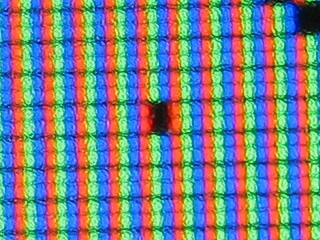
\includegraphics[width=0.35\textwidth]{jk.jpg}}
\caption{Приклад розміщення кристалів}
\end{figure}

\section{Плазмені дисплеї}

Плазмовий дисплей (PDP) - це тип плоскопанельного дисплея, який використовує невеликі комірки, що містять плазму: іонізований газ, який реагує на електричні поля.

Плазмові телевізори були першими великими (понад 32 дюймів по діагоналі) плоскими дисплеями, які були випущені для громадськості. На даний час плазмові дисплеї застаріли, оскільки в більшості, якщо не в усіх аспектах їх замінили OLED-дисплеї. 


Основні недоліки: мерехтіння (через бістабільну природу методу генерації кольору та інтенсивності деякі люди помітять, що плазмові дисплеї мають ефект мерехтіння або мерехтіння з низкою відтінків, інтенсивності та звуження), електроспоживання, не працює також добре на великих висотах понад 2000 метрів через різницю тиску між газами всередині екрана та тиском повітря на висоті. Це може викликати дзижчання.

З переваг можно відзначити більш глибокий чорний ніж у рідкокристалічних, чудовий коефіцієнт контрастності, більш широкі кути огляду, менш помітне розмиття при русі, відмінна однорідність.

\begin{figure}[ht]
\centering{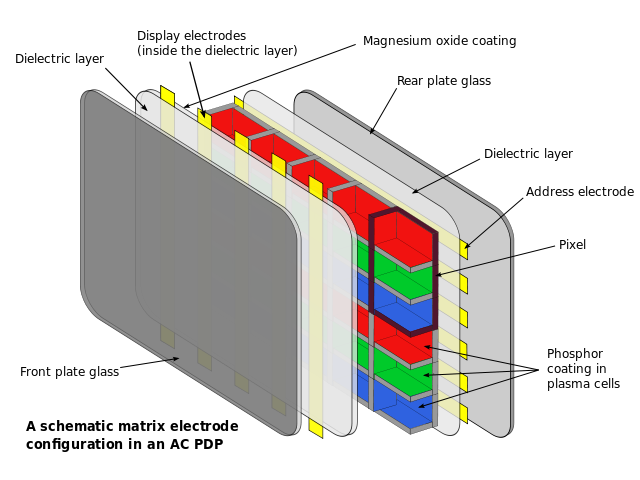
\includegraphics[width=0.5\textwidth]{plasma.png}}
\caption{Будова плазмової панелі}
\end{figure}



\begin{thebibliography}{4}
{\small
\bibitem{book1} \url{http://pps.vtc.vn.ua/} Розділ 3
}
{\small
\bibitem{book2} \url{https://en.wikipedia.org/wiki/Liquid-crystal_display}
}
{\small
\bibitem{book3} \url{https://tech.onliner.by/2020/03/18/displej}
}
{\small
\bibitem{book4} \url{https://en.wikipedia.org/wiki/Cathode-ray_tube}
}
{\small
\bibitem{book5} \url{https://uk.wikipedia.org/wiki/%D0%9F%D0%BB%D0%B0%D0%B7%D0%BC%D0%BE%D0%B2%D0%B8%D0%B9_%D0%B4%D0%B8%D1%81%D0%BF%D0%BB%D0%B5%D0%B9}
}
\end{thebibliography}

\end{document}
